\chapter{Structure of a PASS Description}
\label{PASSStruct}

In this chapter we describe the structure of a PASS specification. The structure of a PASS description consists of the subjects and the messages they exchange.

\section{Informal Description}
\subsection{Subject}
\label{sec: Subject}

Subjects represent the behavior of an active entity. A specification of a subject does not say anything about the technology used to execute the described behavior. Subjects communicate with each other by exchanging messages. Messages have a name and a payload. The name should express the meaning of a message informally and the payloads are the data (business objects) transported. Internal subjects execute local activities such as calculating a price, storing an address etc. External subjects represent interfaces for other business processes.

A subject sends messages to other subjects, receives messages from other subjects, and executes internal actions. All these activities are done in logical order which is defined in a subject's behavior specification.

In the following we use an example for the informal definition of subjects. In the simple scenario of the business trip application, we can identify three subjects, namely the employee as applicant, the manager as the approver, and the travel office as the travel arranger.

In general, there are the following types of subjects:

\begin{itemize}
	\item Fully specified subjects
	\item Multi-subjects
	\item Single subjects
	\item Interface subjects 
\end{itemize}

\subsubsection{Fully specified Subjects}

This is the standard subject type. A subject communicates with other subjects by exchanging messages. Fully specified subjects consists of following components:

\begin{itemize}
	\item Business Objects---Each subject has some business objects. A basic structure of business objects consists of an identifier, data structures, and data elements. The identifier of a business object is derived from the business environment in which it is used. Examples are business trip requests, purchase orders, packing lists, invoices, etc. Business objects are composed of data structures. Their components can be simple data elements of a certain type (e.g., string or number) or even data structures themselves. 
	\item Sent messages---Messages which a subject sends to other subjects. Each message has a name and may transport some data objects as a payload. The values of these payload data objects are copied from internal business objects of a subject.
	\item Received messages---Messages received by a subject. The values of the payload objects are copied to business objects of the receiving subject.
	\item Input Pool---Messages sent to a subjects are deposited in the input pool of the receiving subject. The input pool is a very important organizational and technical concept in this case.
	\item Behavior---The behavior of each subject describes in which logical order it sends messages, expects (receives) messages, and performs internal functions. Messages transport data from the sending to the receiving subject, and internal functions operate on internal data of a subject. 
\end{itemize}


\subsubsection{Multsubjects and Multiprocesses}

Multi-subjects are similar to fully specified subjects. If in a process model several identical subjects are required, e.g. in order to increase the throughput, this requirement can be modeled by a multi-subject. If several communicating subjects in a process model are multi-subjects they can be combined to a multi-process.

In a business process there may be several identical sub-processes that perform certain similar tasks in parallel and independently. This is often the case in a procurement process, when bids from multiple suppliers are solicited. A process or sub-process is therefore executed simultaneously or sequentially multiple times during overall process execution. A set of type-identical, independently running processes or sub-processes are termed multi-process. The actual number of these independent sub-processes is determined at runtime.

Multi-processes simplify process execution, since a specific sequence of actions can be used by different processes. They are recommended for recurring structures and similar process flows. 

An example of a multi-process can be illustrated as a variation of the current booking process. The travel agent should simultaneously solicit up to five bids before making a reservation. Once three offers have been received, one is selected and a room is booked. The process of obtaining offers from the hotels is identical for each hotel and is therefore modeled as a multi-process.

\subsubsection{Single subjects}

Single subjects can be instantiated only once. They are used if for the execution of a subject a resource is required which is only available once.

\subsubsection{Interface Subjects}

Interface subjects are used as interfaces to other process systems. If a subject of a process system sends or receives messages from a subject which belongs to an other process system. These so called interface subjects represent fully described subjects which belong to that other process system. Interface subjects specifications contain the sent messages, received messages and the reference to the fully described subject which they represent.

\subsection{Subject-to-Subject Communication}

After the identification of subjects involved in the process (as process-specific roles), their interaction relationships need to be represented. These are the messages exchanged between the subjects. Such messages might contain structured information—so-called business objects.

The result is a model of the communication relationships between two or more subjects, which is referred to as a \textbf{Subject Interaction Diagram} (SID) or, synonymously, as a Communication Structure Diagram (CSD) (see figure \ref{fig:beispiel-subject-interaction}).

\begin{figure*}[htbp]
	\centering
	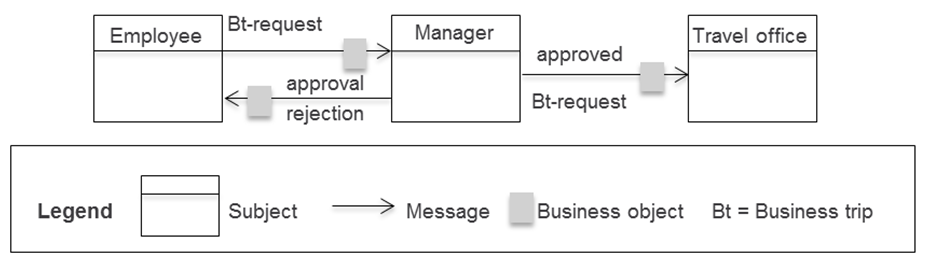
\includegraphics[width=14cm]{20181026-Ontologie-Bilder/Grafiken-Ontologie/SUbject-Interaction/Beispiel-Subject-Interaction}
	\caption[Subject interaction diagram]{Subject interaction diagram for the process 'business trip application'}
	\label{fig:beispiel-subject-interaction}
\end{figure*}

Messages represent the interactions of the subjects during the execution of the process. We recommend naming these messages in such a way that they can be immediately understood and also reflect the meaning of each particular message for the process. In the sample 'business trip application', therefore, the messages are referred to as 'business trip request', 'rejection', and 'approval'.

Messages serve as a container for the information transmitted from a sending to a receiving subject. There are two options for the message content:

\begin{itemize}
	\item 	Simple data types---Simple data types are string, integer, character, etc. In the business trip application example, the message 'business trip request' can contain several data elements of type string (e.g., destination, reason for traveling, etc.), and of type number (e.g., duration of trip in days).
	\item Business Objects---Business Objects in their general form are physical and logical 'things' that are required to process business transactions. We consider data structures composed of elementary data types, or even other data structures, as logical business objects in business processes. For instance, the business object 'business trip request' could consist of the data structures 'data on applicants', 'travel data', and 'approval data' with each of these in turn containing multiple data elements.
\end{itemize}

\subsection{Message Exchange}

In the previous subsection, we have stated that messages are transferred between subjects and have described the nature of these messages. What is still missing is a detailed description of how messages can be exchanged, how the information they carry can be transmitted, and how subjects can be synchronized. These issues are addressed in the following sub-sections.

\subsubsection{Synchronous and Asynchronous Exchange of Messages}

In the case of synchronous exchange of messages, sender and receiver wait for each other until a message can be passed on. If a subject wants to send a message and the receiver (subject) is not yet in a corresponding receive state, the sender waits until the receiver is able to accept this message. Conversely, a recipient has to wait for a desired message until it is made available by the sender.

The disadvantage of the synchronous method is a close temporal coupling between sender and receiver. This raises problems in the implementation of business processes in the form of workflows, especially across organizational borders. As a rule, these also represent system boundaries across which a tight coupling between sender and receiver is usually very costly. For long-running processes, sender and receiver may wait for days, or even weeks, for each other.

Using asynchronous messaging, a sender is able to send anytime. The subject puts a message into a message buffer from which it is picked up by the receiver. However, the recipient sees, for example, only the oldest message in the buffer (in case the buffer is implemented as FIFO or LIFO storage) and can only accept this particular one. If it is not the desired message, the receiver is blocked, even though the message may already be in the buffer, but in a buffer space that is not visible to the receiver. To avoid this, the recipient has the alternative to take all of the messages from the buffer and manage them by himself. In this way, the receiver can identify the appropriate message and process it as soon as he or she needs it. In asynchronous messaging, sender and receiver are only loosely coupled. Practical problems can arise due to the in reality limited physical size of the receive buffer, which does not allow an unlimited number of messages to be recorded. Once the physical boundary of the buffer has been reached due to high occupancy, this may lead to unpredictable behavior of workflows derived from a business process specification. To avoid this, the input-pool concept has been introduced in PASS. Nevertheless, the number of messages must always be limited, as a business process must have the capacity to handle all messages to maintain some sort of service level.


\subsubsection{Exchange of Messages via the Input Pool}
\label{sec: inputpool}

To solve the problems outlined in asynchronous message exchange, the input pool concept has been developed. Communication via the input pool is considerably more complex than previously shown; however, it allows transmitting an unlimited number of messages simultaneously. Due to its high practical importance, it is considered as a basic construct of PASS.

Consider the input pool as a mail box of work performers, the operation of which is specified in detail. Each subject has its own input pool. It serves as a message buffer to temporarily store messages received by the subject, independent of the sending communication partner. The input pools are therefore inboxes for flexible configuration of the message exchange between the subjects. In contrast to the buffer in which only the front message can be seen and accepted, the pool solution enables picking up (i.e. removing from the buffer) any message. For a subject, all messages in its input pool are visible.

The input pool has the following configuration parameters (see figure \ref{fig:input-pool}):

\begin{itemize}
	\item Input-pool size---The input-pool size specifies how many messages can be stored in an input pool, regardless of the number and complexity of the message parameters transmitted with a message. If the input pool size is set to zero, messages can only be exchanged synchronously.
	\item Maximum number of messages from specific subjects---For an input pool, it can be determined how many messages received from a particular subject may be stored simultaneously in the input pool. Again, a value of zero means that messages can only be accepted synchronously.
	\item Maximum number of messages with specific identifiers---For an input pool, it can be determined how many messages of a specifically identified message type (e.g., invoice) may be stored simultaneously in the input pool, regardless of what subject they originate from. A specified size of zero allows only for synchronous message reception.
	\item Maximum number of messages with specific identifiers of certain subjects---For an input pool, it can be determined how many messages of a specific identifier of a particular subject may be stored simultaneously in the input pool. The meaning of the zero value is analogous to the other cases.
\end{itemize}

\begin{figure*}[htbp]
	\centering
	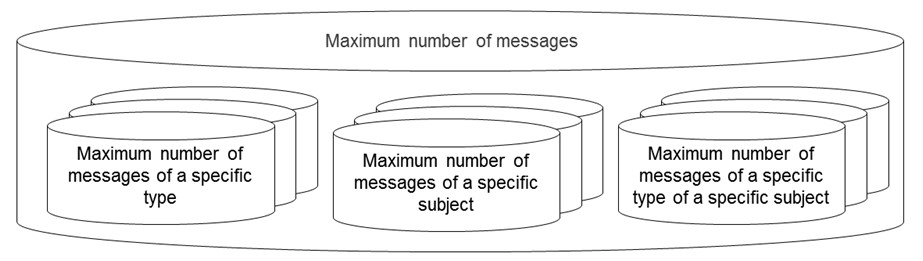
\includegraphics[width=12cm]{20181026-Ontologie-Bilder/Grafiken-Ontologie/SUbject-Interaction/input-pool-informal.jpg}
	\caption[Input Pool]{Configuration of Input Pool Parameters}
	\label{fig:input-pool}
\end{figure*}

By limiting the size of the input pool, its ability to store messages may be blocked at a certain point in time during process runtime. Hence, messaging synchronization mechanisms need to control the assignment of messages to the input pool. Essentially, there are three strategies to handle the access to input pools:

\begin{itemize}
	\item Blocking the sender until the input pool’s ability to store messages has been reinstated---Once all slots are occupied in an input pool, the sender is blocked until the receiving subject picks up a message (i.e. a message is removed from the input pool). This creates space for a new message. In case several subjects want to put a message into a fully occupied input pool, the subject that has been waiting longest for an empty slot is allowed to send. The procedure is analogous if corresponding input pool parameters do not allow storing the message in the input pool, i.e., if the corresponding number of messages of the same name or from the same subject has been put into the input pool.
	\item Delete and release of the oldest message---In case all the slots are already occupied in the input pool of the subject addressed, the oldest message is overwritten with the new message.
	\item Delete and release of the latest message---The latest message is deleted from the input pool to allow depositing of the newly incoming message. If all the positions in the input pool of the addressed subject are taken, the latest message in the input pool is overwritten with the new message. This strategy applies analogously when the maximum number of messages in the input pool has been reached, either with respect to sender or message type.
\end{itemize}

\section{OWL Description}
\label{OWL-DescriptionSID}

The various building blocks of a PASS description and their relations are defined in an ontology. The following figure \ref{fig:20171217-passprocessmodellelement} gives an overview of the structure of the PASS specifications.   

\begin{figure*}[htbp]
	\centering
	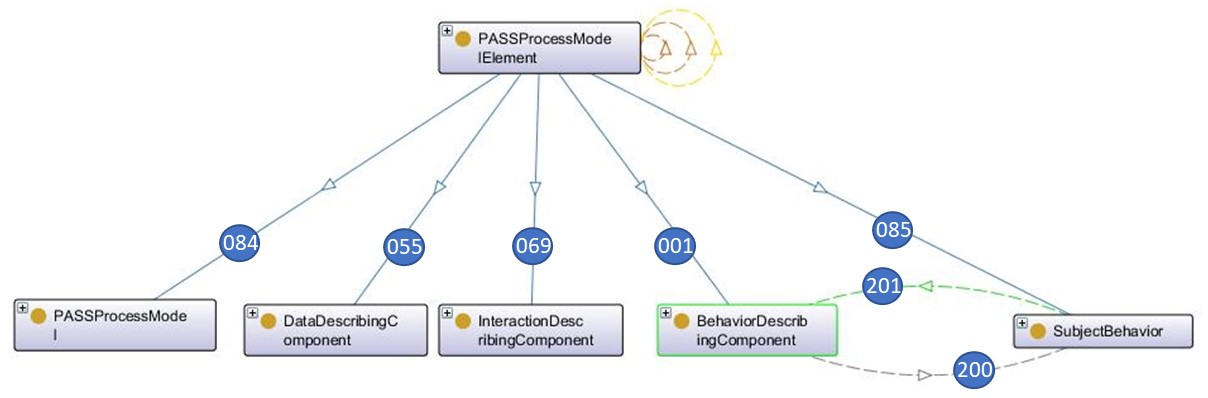
\includegraphics[width=0.9\linewidth]{20181026-Ontologie-Bilder/Grafiken-Ontologie/SUbject-Interaction/20171217-PASSProcessModellElement}
	\caption[Elements of PASS Process Models]{Elements of PASS Process Models}
	\label{fig:20171217-passprocessmodellelement}
\end{figure*}

The class \texttt{PASSProcessModelElement} has five subclasses (subclass relations 084, 055, 069, 001 and 085 in figure \ref{fig:20171217-passprocessmodellelement}). Only the classes \texttt{PASSProcessModel}, \texttt{DataDescriptionCOmponent}, \texttt{InteractionDescribingComponent} are used for defining the structural aspects of a process specification in PASS. The classes \texttt{BehaviorDescribingComponent} and \texttt{SubjectBehavior} define the dynamic aspects. In which sequences messages are sent and received or internal actions are executed. These dynamic aspects are considered in detail in the next chapter. 

\subsection{PASS Process Model}

The central entities of a PASS process model are subjects which represents the active elements of a process and the messages they exchange. Messages transport data from one subject to others (payload). Figure \ref{fig:20181217-passprocessmodel} shows the corresponding ontology for the PASS process models.

\begin{figure*}[htbp]
	\centering
	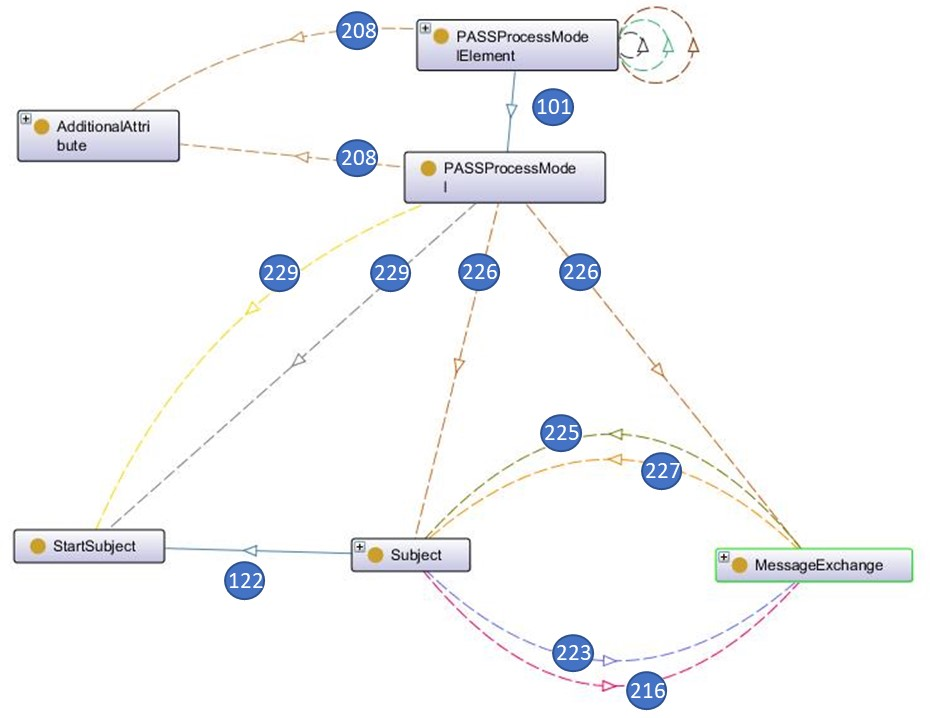
\includegraphics[width=1.0\linewidth]{20181026-Ontologie-Bilder/Grafiken-Ontologie/SUbject-Interaction/20181217-PASSProcessModel}
	\caption[PASS Process Modell]{PASS Process Modell}
	\label{fig:20181217-passprocessmodel}
\end{figure*}

\texttt{PASSProcessModelElements} and \texttt{PASSProcessModells} have a name. This is described with the property \texttt{hasAdditionalAttribute} (property 208 in \ref{fig:20171217-passprocessmodellelement}). The class subject and the class \texttt{MessageExchange} have the relation \texttt{hasRelation} \texttt{toModelComponent} to the class \texttt{PASSProcessModel} (property 226 in \ref{fig:20171217-passprocessmodellelement}). The properties \texttt{hasReceiver} and \texttt{hasSender} express that a message has a sending and receiving subject (properties 225 and 227 in \ref{fig:20171217-passprocessmodellelement}) whereas the properties \texttt{hasOutgoingMessageExchange} and \texttt{hasIncomingMessageExchange} define which messages are sent or received by a subject. Property \texttt{hasStartSubject} (property 229 in \ref{fig:20171217-passprocessmodellelement}) defines a start subject for a \texttt{PASSProcessModell}. A start subject is a subclass of the class subject (subclass relation 122 in \ref{fig:20171217-passprocessmodellelement}).

\subsection{Data Describing Component}

Each subject encapsulate data (business objects). The values of these data elements can be transferred to other subjects. The following figure \ref{fig:20181218-data} shows the ontology of this part of the PASS-ontology.

\begin{figure}[htbp]
	\centering
	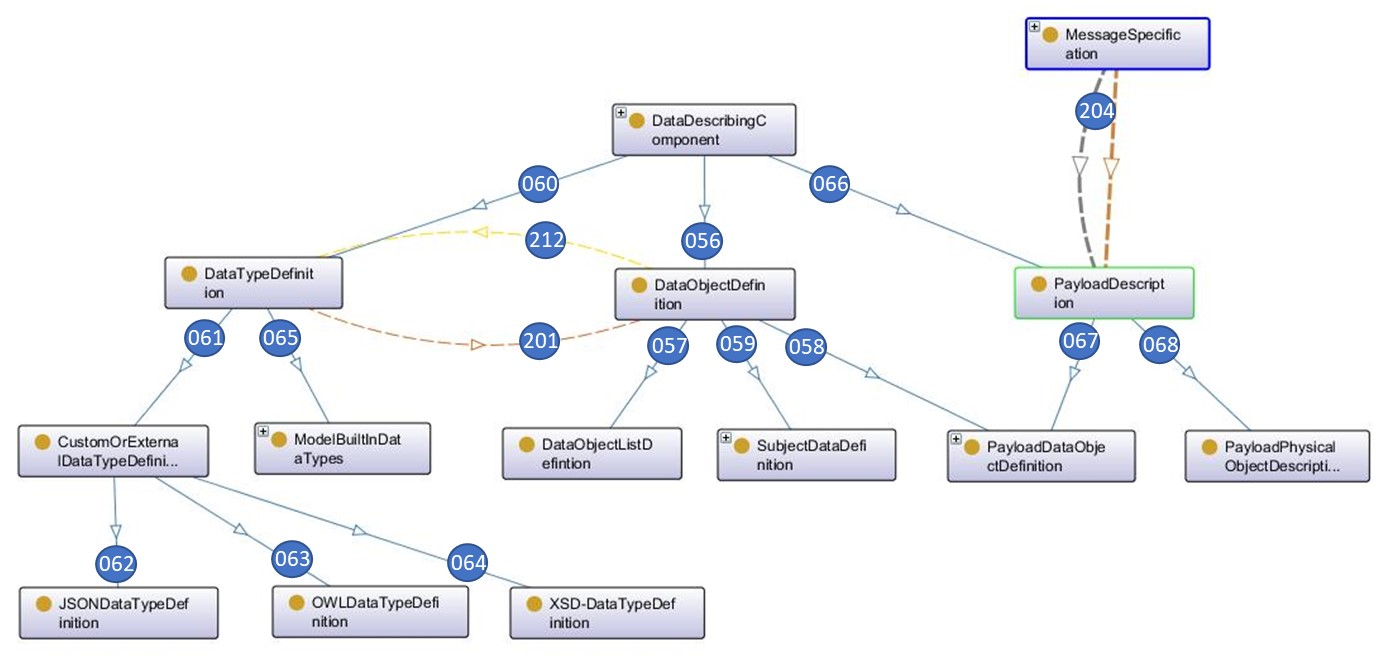
\includegraphics[width=0.9\linewidth]{20181026-Ontologie-Bilder/Grafiken-Ontologie/SUbject-Interaction/20181218-Data}
	\caption[Data Description Component]{Data Description Component}
	\label{fig:20181218-data}
\end{figure}

Three subclasses are derived from the class \texttt{DtadescribingCombonent} (in figure \ref{fig:20181218-data} are these the relations 060, 056 and 066). The subclass \texttt{PayLoadDescription} defines the data tranported by messages. The relation of \texttt{PayloadDescriptions} to messages is defined by the property \texttt{ContainsPayloadDescription} (in figure \ref{fig:20181218-data} number 204).

There are two types of payloads. The class \texttt{PayloadPhysicalObjectDescription} is used if a message will be later implemented by a physical transport like a parcel. The class \texttt{PayLoadDataObjectDefinition} is used to transport normal data (Subclass relations 068 and 67 in figure \ref{fig:20181218-data}). These payload objects are also a subclass of the class \texttt{DataObjectDefinition} (Subclass relation 058 in figure \ref{fig:20181218-data}).

Data objects have a certain type. Therefore class \texttt{DataObjectDefinition} has the relation \texttt{hasDatatype} to class \texttt{DataTypeDefinition} (property 212 in figure\ref{fig:20181218-data}). Class \texttt{DataTypeDefinition} has two subclasses (subclass relations 061 and 065 in figure \ref{fig:20181218-data}). The subclass \texttt{ModelBuiltInDataTypes} are user defined data types whereas the class \texttt{CustomOfExternalDataTypeDefinition} is the superclass of JSON, OWL or XML based data type definitions(subclass relations 062, 63 and 064 in figure \ref{fig:20181218-data}).

\subsection{Interaction Describing Component}

The following figure \ref{fig:ontogrsubjectinteraction} shows the subset of the classes and properties required for describing the interaction of subjects. 

\begin{figure*}[htbp]
	\centering
	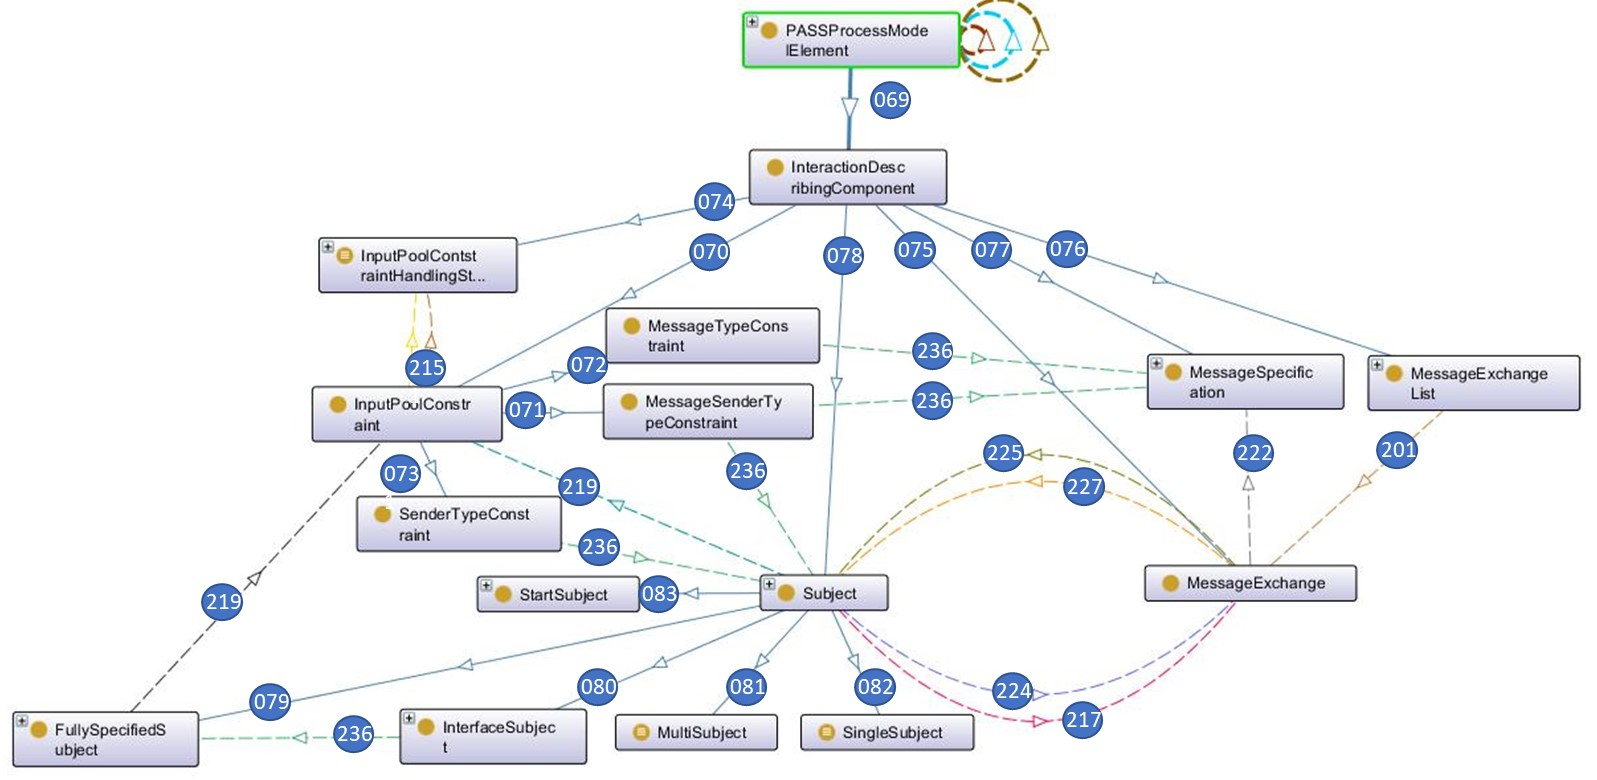
\includegraphics[width=1.0\linewidth]{20181026-Ontologie-Bilder/Grafiken-Ontologie/SUbject-Interaction/OntoGrSubjectInteraction}
	\caption[Subject Interaction Diagram]{Subject Interaction Diagram}
	\label{fig:ontogrsubjectinteraction}
\end{figure*}

The central classes are \texttt{Subject} and \texttt{MessageExchange}. Between these classes are defined the properties \texttt{hasIncomingTransition} (in figure \ref{fig:ontogrsubjectinteraction} number 217) and \texttt{hasOutgoingTransition} (in figure \ref{fig:ontogrsubjectinteraction} number 224). This properties defines that subjects have incoming and outgoing messages. Each message has a sender and a receiver (in figure \ref{fig:ontogrsubjectinteraction} number 227 and number 225). Messages have a type. This is expressed by the property \texttt{hasMessageType} (in figure \ref{fig:ontogrsubjectinteraction} number 222). Instead of the property 222 a message exchange may have the property 201 if a list of messages is used instead of a single message.

Each subject has an input pool. Input pools have three types of constraints (see section \ref{sec: inputpool}). This is expressed by the property references  (in figure \ref{fig:ontogrsubjectinteraction} number 236) and \texttt{InputPoolConstraints} (in figure \ref{fig:ontogrsubjectinteraction} number 219). Constraints which are related to certain messages have references to the class \texttt{MessageSpecification}.

There are four subclasses of the class \texttt{subject} (in figure \ref{fig:ontogrsubjectinteraction} number 079, 080, 081 and 082). The specialties of these subclasses are described in section \ref{sec: Subject}. A class \texttt{StartSubject} (in figure \ref{fig:ontogrsubjectinteraction} number 83) which is a subclass of class subject denotes the subject in which a process instance is started.

All other relations are subclass relations. The class \texttt{PASSProcessModelElement} is the central PASS class. From this class all the other classes are derived (see next sections). From class \texttt{InteractionDescribingCOmponent} all the classes required for describing the structure of a process system are derived.

\section{ASM Description}

In this chapter only the structure of a PASS model is considered. Execution has not been considered. Because ASM only considers execution aspects in this chapter an ASM specification of the structural aspects does not make sense. The execution semantic is part of chapter 4.
